%% LyX 1.6.2 created this file.  For more info, see http://www.lyx.org/.
%% Do not edit unless you really know what you are doing.
%\documentclass[english]{article}
%\usepackage[T1]{fontenc}
%\usepackage[latin9]{inputenc}

%\usepackage{babel}

%\begin{document}

\chapter{Arches}

\section{Introduction}
% please fix....
The ARCHES component was initially designed for predicting the
potential hazard of an explosive device immersed in or near a pool
fire of transportation fuel.  Since then, this component has been
extended to solve many industrially relevant problems such as
industrial flares, oxy-coal combustion processes, and fuel
gasification.

Given the wide range of length and time scales that are present in these examples, ARCHES utilizes models for bridging the molecular (micro) scales to the full, large (macro) scales.  More to come....

The ARCHES component solves the conservative, finite volume, low-mach formulation of the Navier-Stokes equation with a pressure projection that includes the effect of variable density, reaction, and many modes of heat transfer including radiation.  

\section{Governing Equations}
%
The essential governing equations for the Arches component, written in
finite volume form, include the mass balance, momentum balance,
mixture fraction balance, and energy balance equations. Using a
bold-face symbol to represent a vector quantity, the equations are:
\begin{enumerate}
\item The mass balance, \begin{equation}
\int_{V}\frac{\partial\rho}{\partial t}dV+\oint_{S}\rho\mathbf{u}\cdot d\mathbf{S}=0\;,\label{eqn:mass_balance}\end{equation}
 where $\rho$ is density and $\mathbf{u}$ is the velocity vector. 
\item The momentum balance, \begin{equation}
\int_{V}\frac{\partial\rho\mathbf{u}}{\partial t}dV+\oint_{S}\rho\mathbf{uu}\cdot d\mathbf{S}=\oint_{S}\tau\cdot d\mathbf{S}-\int_{V}\nabla pdV+\int_{V}\rho\mathbf{g}dV\;,\label{eqn:mom_balance}\end{equation}
 where $\tau$ is the deviatoric stress tensor defined as $\tau_{ij}=2\mu S_{ij}-\frac{2}{3}\mu\frac{\partial u_{k}}{\partial x_{k}}\delta_{ij}$,
the second isotropic term in $\tau_{ij}$ is absorbed into the pressure
projection for the current low-Mach scheme, and $S_{ij}=\frac{1}{2}\left(\frac{\partial u_{i}}{\partial x_{j}}+\frac{\partial u_{j}}{\partial x_{i}}\right)$.
Also in Equation \ref{eqn:mom_balance}, $\mathbf{g}$ is the gravitational
body force and $p$ is pressure. 
\item The mixture fraction balance, \begin{equation}
\int_{V}\frac{\partial\rho f}{\partial t}dV+\oint_{S}\rho\mathbf{u}f\cdot d\mathbf{S}=\oint_{S}D\nabla f\cdot d\mathbf{S}\;,\label{eqn:species_balance}\end{equation}
 where $f$ is the mixture fraction and a Fick's law form of the diffusion
term assuming equal diffusivities results in a single diffusion coefficient,
$D$. 
\item The thermal energy balance, \begin{equation}
\int_{V}\frac{\partial\rho h}{\partial t}dV+\oint_{S}\rho\mathbf{u}h\cdot d\mathbf{S}=\oint_{S}k\nabla h\cdot d\mathbf{S}-\oint_{S}q\cdot d\mathbf{S}\;,\label{eqn:heat_balance}\end{equation}
 where $h$ is the sum of the chemical plus sensible enthalpy, $q$
is the radiative flux, a Fourier's law form of the conduction term
is used with a diffusion coefficient, $k$, and the pressure term
is neglected. 
\end{enumerate}
These equations are solved in an LES context, meaning filters are
applied to the equations. Here, we use Favre filtering, defined as
\[
\overline{\phi}=\frac{\overline{\rho\phi}}{\overline{\rho}},\]
 to isolate the density in the filtered equations. The filtering operations
result in the classic turbulence closure problem and thus models are
required. 

Consider a control volume, $V$, with surface area $S$.  Because the equations will be  solved on a computational grid, one can safely assume that the the control volume has $N$ faces, where unique faces are identified with their index, $k$.  The discussion is further simplified by only considering cubic volumes with length $h$.  
Given the cubic control volume, a surface-filtered field for a variable $\phi$ is defined as $\overline{\phi}^{(j)}(\mathbf{x})$, where the variable is filtered on a plane in the $x_j$ orthogonal direction.  Then, for any surface, $k$, the field is sampled at the face centered location.  For example, if $j=1$, the surface-filtered quantity is
%
\begin{equation}
\overline{\phi}^{2d, (1)}(\mathbf x) = \frac{1}{h^2} \int_{x_2 - h/2}^{x_2 + h/2}  \int_{x_3 - h/2}^{x_3 + h/2} \phi(\mathbf x') dx_2' dx_3' \; .
\end{equation} 
%
The volume average follows as
%
\begin{equation}
\overline{\phi}^{3d} (\mathbf x) = \frac{1}{h^3} \int_{x_1 - h/2}^{x_1 + h/2} \int_{x_2 - h/2}^{x_2 + h/2}  \int_{x_3 - h/2}^{x_3 + h/2} \phi(\mathbf x') dx_1' dx_2' dx_3' \; .
\end{equation}
%
The bars over the variable, $\phi$, are labeled with `2d' and `3d' superscripts to distinguish between the two filters.  Pope \cite{Pope179} identifies the proceeding definitions as using the ``anisotropic box" filter kernel where the resultant variables are simply averages over the intervals $x_j - \frac{1}{2}h < x_j' < x_j + \frac{1}{2}h$. 

For convenience in isolating density in the filtered equations, a Favre-filtered quantity is defined for an arbitrary variable, $\varphi$, as 
%
\begin{equation}\label{eqn:favre_surf}
\widetilde{\varphi}^{2d} \equiv \frac{\overline{\rho \varphi}^{2d}}{\overline{\rho}^{2d}} \; ,
\end{equation}
%
and
%
\begin{equation}\label{eqn:favre_vol}
\widetilde{\varphi}^{3d} \equiv \frac{\overline{\rho \varphi}^{3d}}{\overline{\rho}^{3d}} \;.
\end{equation}
%
Because the 2d and 3d filters are explicitly defined, this convention is slightly different than what is normally observed in the literature.  Most literature, however, derives the filtered equations from the finite difference equations rather than the finite volume equations.  Thus, using $\overline{\rho}^{2d}$ and $\overline{\rho}^{3d}$ in Equations \ref{eqn:favre_surf} and \ref{eqn:favre_vol} to stress surface and volume filtered densities are appropriate for the present discussion.

The previous definitions are applied to the integral forms of the governing equations to obtain the Favre-filtered LES equations.  Nevertheless, there are terms in the Favre-filtered equations that cannot be solved.  These include the surface filtered convection of momentum, $\widetilde{u_i u}^{2d}_j$, the surface filtered convection of mixture fraction, $\widetilde{u_j f}^{2d}$, and the surface filtered convection of enthalpy, $\widetilde{u_j h}^{2d}$.  

For the filtered velocity product, $\overline{\rho}^{2d} \; \widetilde{ u_i u}^{2d}_j$, a subgrid stress tensor is defined as, 
%
\begin{equation}\label{eqn:tau_sgs}
\tau^{sgs}_{ij} = \widetilde{u_i u}^{2d}_j - \widetilde{u}^{2d}_i \widetilde{u}^{2d}_j \; .
\end{equation}
%
Similarly, subgrid diffusion terms are defined for mixture fraction and enthalpy, 
%
\begin{eqnarray}
\mathcal{J}^{f}  = \widetilde{u_j f}^{2d} - \widetilde{u}^{2d}_j \widetilde{f}^{2d} \;, \\
\mathcal{J}^{h} = \widetilde{u_j h}^{2d} - \widetilde{u}^{2d}_j \widetilde{h}^{2d} \; .\\
\end{eqnarray}

Using these definitions, the final form of the Favre-filtered equations is
%
\begin{enumerate}
\item The filtered mass balance, 
%
\begin{equation}\label{eqn:filtered_mass_balance}
\frac{d}{d t} \left(\widetilde{\rho}^{3d} \right)   + \frac{S_k}{V} n_{kj} \left( \overline{\rho}^{2d} \; \widetilde{u}^{2d}_j \right) = 0 \; .
\end{equation}
%
\item The filtered momentum balance, 
%
\begin{equation}\label{eqn:filtered_mom_balance}
\frac{d}{d t} \left( \overline{\rho}^{3d} \; \widetilde{u}^{3d}_i \right) = \frac{S_{k}}{V} n_{kj}\left( -\overline{\rho}^{2d} \; \widetilde{u}^{2d}_i\widetilde{u}^{2d}_j + \overline{\tau}^{2d}_{ij} + \tau^{sgs}_{ij} - \overline{p}^{2d} \delta_{ij} \right) + \overline{\rho}^{3d} \; g_i  \; .
\end{equation}
%
\item The filtered mixture fraction balance,
%
\begin{equation}\label{eqn:filtered_mixfrac_balance}
\frac{d}{d t} \left( \overline{\rho}^{3d} \; \widetilde{f}^{3d} \right) = \frac{S_k}{V} n_{kj} \left( -\overline{\rho}^{2d} \; \widetilde{u}^{2d}_j \widetilde{f}^{2d} + D \nabla \overline{f}^{2d} + \mathcal{J}^{f} \right) \; .
\end{equation}
%
%
\item The filtered thermal energy balance, 
%
\begin{equation}\label{eqn:filtered_heat_balance}
\frac{d}{d t} \left( \overline{\rho}^{3d} \; \widetilde{h}^{3d} \right) = \frac{S_{k}}{V} n_{kj} \left( -\overline{\rho}^{2d} \; \widetilde{u_j}^{2d}\widetilde{h}^{2d} + k \nabla \overline{h}^{2d}  - \overline{q}^{2d}  + \mathcal{J}^h \right) \; .
\end{equation}
%
\end{enumerate}
The subgrid momentum stress, $\tau_{ij}^{sgs}$, the subgrid mixture fraction dissipation, $\mathcal{J}^{f}$, and the subgrid heat dissipation, $\mathcal{J}^{h}$, contain the unresolved or subgrid action of the turbulence on the transported quantities.  Since these terms arise from definitions, models are introduced to include the subgrid effects that they represent.  These models are discussed next.

\subsection{Subgrid Turbulence Models}
%
The construction of both $\mathcal{J}^f$ and $\mathcal{J}^{h}$ is relatively straight forward. Invoking an ``eddy-viscosity" modeling concept, the subgrid transport due to turbulent advection is treated as an enhanced diffusion term for the unclosed terms listed above.   That is, the subgrid mixture fraction dissipation and subgrid enthalpy dissipation are respectively written as, 
%
\begin{equation}
\mathcal{J}^{f} = D_{t} \frac{\partial \overline{f}^{2d}}{\partial x_j} \; , 
\end{equation}
%
and 
%
\begin{equation}
\mathcal{J}^{h} = k_{t} \frac{\partial \overline{h}^{2d}}{\partial x_j} \; .
\end{equation}
%
To model $D_{t}$ and $k_{t}$, constant turbulent Schmidt ($Sc_t$),
%
\begin{equation}\label{eqn:subgrid_mixfrac}
Sc_{t} = \frac{1}{\rho} \frac{\mu_t}{D_t} \; ,
\end{equation}
%
and Prandlt ($Pr_t$), 
%
\begin{equation}\label{eqn:subgrid_enthalpy}
Pr_{t} = \frac{1}{\rho} \frac{\mu_t}{k_t} \; ,
\end{equation}
%
numbers are assumed with where $\mu_t$ is a turbulent viscosity.  Following Pitsch and Steiner \cite{pitsch2000}, the values of the turbulent Schmidt and Prandlt number are taken as $Sc_t = Pr_t = 0.4$, which is consistent with a unity Lewis number assumption.  

For the subgrid scale stress tensor, $\tau^{sgs}_{ij}$, two common LES turbulence closure models are the constant coefficient Smagorinsky model \cite{Smagorinsky178} and the dynamic coefficient Smagorinsky model \cite{Moin158}.  As with the scalar subgrid modeling terms, the eddy viscosity model is again invoked for $\tau^{sgs}_{ij}$.  Defining the deviatoric subgrid stress tensor as, 
%
\begin{equation}
\tau^{d, sgs}_{ij} = \tau^{sgs}_{ij} - \frac{1}{3}\tau^{sgs}_{kk} \delta_{ij}, 
\end{equation}
%
the subgrid stress is taken as,
%
\begin{equation}
\tau_{ij}^{d, sgs} \approx -2 \nu_t \overline{S}_{ij} = -2 (C_s \Delta)^2 |\overline{S}|\overline{S}_{ij} \; , 
\end{equation}
%
where $\Delta$ is the filter width, $\nu_t$ is the eddy viscosity and $|\overline{S}| \equiv (2\overline{S}_{ij}\overline{S}_{ij})^{1/2}$.  For the Smagorinsky model,  $C_s \approx 2$  depending on the filter type, numerical method, and flow configuration \cite{Pope179}.  

For the dynamic Smagorinsky model, $C_s$ is computed by taking a least squares approach to determining the length scale \cite{Lilly180},
%
\begin{equation} \label{eqn:cs_eqn}
(C_s \Delta)^2 = \frac{ \left< \mathcal{L}_{ij} M_{ij} \right>}{ \left< M_{ij}M_{ij} \right> } \; ,
\end{equation}
%
where
%
%
\begin{equation}
\mathcal{L}_{ij} = 2( C_s \Delta)^2 \widehat{ |\overline{S} | \overline{S} }_{ij} - 
   2( C_s \widehat{\Delta})^2 \widehat{ |\overline{S}} | \widehat{\overline{S}}_{ij} \; ,
\end{equation}
%   
and
\begin{equation}
M_{ij} \equiv 2 \left( \widehat{ | \overline{S} | \overline{S} }_{ij} - \alpha^2 |\widehat{\overline{S}}|\widehat{\overline{S}}_{ij} \right) \; .
\end{equation} 
%
The hat defines an explicit test filter and the angled brackets in
Equation \ref{eqn:cs_eqn} conceptually represent an averaging over a
homogeneous region of space that, experience has shown, is necessary
for stability.  Experience has also shown that averaging over the test
filter width is adequate and the filter width ratio, $\alpha =
\widehat{\Delta}/\Delta$, is usually taken to be 2.

\subsection{Subgrid Momentum Dissipation}
%%
Addressing the momentum closure involves finding a suitable model for the subgrid scale stress tensor, $\tau^{sgs}_{ij}$.  Two common LES turbulence closure models are examined: the constant coefficient Smagorinsky model and the dynamic coefficient Smagorinsky model.  
%%
In LES modeling, field variables are decomposed into a spatially
filtered field and a residual component, $u = \overline{u} + u'$.
This decomposition is known as a Leonard decomposition.  While
seemingly similar to a Reynolds decomposition used in Reynolds
Averaged Navier-Stokes (RANS) models, the Leonard decomposition has
the property that the filtered residual component is generally not
equal to zero, $\overline{u'} \neq 0$.  As a result, the subgrid
stress term contains several terms,
%%%
\begin{eqnarray}
\tau_{ij}^{sgs} = \overline{ \left(\overline{u}_i + u_i' \right) \left(\overline{u}_i + u_i' \right)} - \overline{u}_i \overline{u}_j \; , \; \; \; \; \; \; \; \; \; \; \; \; \; \;  \; \; \nonumber \\
= \underbrace{\overline{\overline{u}_i \overline{u}_j} - \overline{u}_i \overline{u}_j}_{L_{ij}}  + 
   \underbrace{\overline{\overline{u}_i {u}_j'} + \overline{{u}_i' \overline{u}_j}}_{C_{ij}} + 
   \underbrace{ \overline{u_i' + u_j'} }_{R_{ij}} \; , 
\end{eqnarray}
%
referred to as the Leonard stress, the cross stresses, and the
Reynolds stress respectively.

It is useful to consider the physical interpretation of the various
components of the stress. The Leonard term is responsible for
filtering and projecting the nonlinear interactions of the resolved
components back to the finite LES space.  This is a correction to the
resolved advective term in accordance with the stated explicit filter
used to derive the LES equations. It does not account for aliasing
errors. The first cross term represents advection of the resolved
field by turbulent fluctuations. The second cross term represents the
advection of subgrid scales by the resolved field. The Reynolds stress
is familiar from RANS and represents the advection of subgrid scales
by turbulent fluctuations.

As with the scalar subgrid modeling terms, the eddy viscosity model is
again invoked for $\tau^{sgs}_{ij}$.  The most common eddy viscosity
model in LES is the Smagorinsky model \cite{Smagorinsky178}.  Defining
the deviatoric subgrid stress tensor as,
%%
\begin{equation}
\tau^{d, sgs}_{ij} = \tau^{sgs}_{ij} - \frac{1}{3}\tau^{sgs}_{kk} \delta_{ij}, 
\end{equation}
%%
the subgrid stress is approximated by,
%%
\begin{equation}
\tau_{ij}^{d, sgs} \approx -2 \nu_t \overline{S}_{ij} = -2 (C_s \Delta)^2 |\overline{S}|\overline{S}_{ij} \; , 
\end{equation}
%%
where, $\Delta$ is the filter width, $\nu_t$ is the eddy viscosity, $|\overline{S}| \equiv (2\overline{S}_{ij}\overline{S}_{ij})^{1/2}$, and typically $C_s \approx 2$  depending on the filter type, numerical method, and flow configuration \cite{Pope179}. This model is basically identical to Prandtl's mixing length model with $l = C_s \Delta$.

The dynamic procedure \cite{Germano74, Moin158} eliminates the need to
specify the model constant, $C_s$, a priori, with the basic assumption
that the constant is the same for two different filter scales. The
smaller scale is historically referred to as the ``grid scale" (though
the filter width need not equal the grid spacing, $\Delta \geq h$)),
and the larger scale is referred to as the ``test scale".  Implicit in
this assumption is the requirement that both scales lie within the
inertial subrange.

Defining the deviatoric residual stress tensor as, 
\begin{equation}
T_{ij}^d = T_{ij} - \frac{1}{3} T_{kk}\delta_{ij} \;,
\end{equation}
the residual stress at the test scale is given by,
%%
\begin{equation}\label{eqn:res_stress}
T_{ij}^{d} \equiv \overline{\widehat {u_i u_j}} - \overline{\widehat{u}}_i \overline{\widehat{u}}_j \approx -2(C_s \widehat{\Delta})^2 |\widehat{\overline{S}}| \widehat{\overline{S}}_{ij} \; .
\end{equation}
%%
where $\widehat{\Delta}$ is the test filter width and the hat defines an explicit test filter. By test filtering Equation \ref{eqn:tau_sgs} and combining this with \ref{eqn:res_stress}, one can construct the Leonard term, $\mathcal{L}_{ij}$. This is also known as the ``Germano identity",
%%
\begin{equation}
\mathcal{L}_{ij} = T_{ij} - \widehat{ \tau^{sgs}}_{ij} =  \overline{\widehat {u_i u_j}} - \overline{\widehat{u}}_i \overline{\widehat{u}}_j \; .
\end{equation}
%%
Notice that the Leonard term is directly computable from resolved LES quantities. By restating the Smagorinsky model in terms of the Germano identity, one ends up with an over-determined system of equations for the unknown, $C_s$,
%%
\begin{equation}
\mathcal{L}_{ij} = 2( C_s \Delta)^2 \widehat{ |\overline{S} | \overline{S} }_{ij} - 
   2( C_s \widehat{\Delta})^2 \widehat{ |\overline{S}} | \widehat{\overline{S}}_{ij} \; .
\end{equation}
%%   
Although we have pulled $C_s$ out of the test filtering operation of the subgrid stress, this approximation yields acceptable results. In practice, one takes a least squares approach to determining the length scale \cite{Lilly180},
%%
\begin{equation} \label{eqn:cs_eqn}
(C_s \Delta)^2 = \frac{ \left< \mathcal{L}_{ij} M_{ij} \right>}{ \left< M_{ij}M_{ij} \right> } \; ,
\end{equation}
%%
where
%%
\begin{equation}
M_{ij} \equiv 2 \left( \widehat{ | \overline{S} | \overline{S} }_{ij} - \alpha^2 |\widehat{\overline{S}}|\widehat{\overline{S}}_{ij} \right) \; .
\end{equation} 
%%
The only model parameter, then, is the filter width ratio, $\alpha = \widehat{\Delta}/\Delta$, usually taken to be 2.

The angled brackets in Equation \ref{eqn:cs_eqn} conceptually represent averaging over a homogeneous region of space which, experience has shown, is necessary for stability. We have found that averaging over the test filter width is adequate.
%%
With these implementation practices, the dynamic model is generally robust. The implementation can be made more efficient by computing the constant roughly every 10 time steps (based on the advective CFL), and only for the first Runge-Kutta step.

\subsection{LES Algorithm}\label{Sec:LES_Algorithm}

%
%% Staggered Grid
\begin{wrapfigure}{r}{.5\textwidth}
 \begin{center}
   \vspace{-35pt}
%   \scalebox{.85}{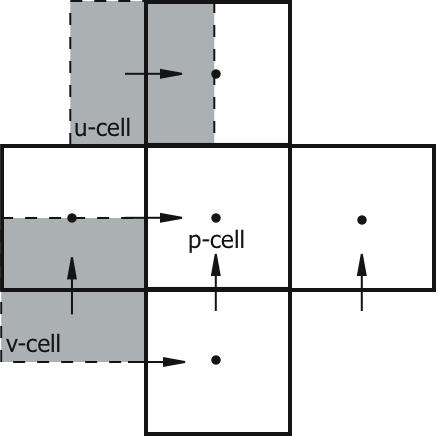
\includegraphics{staggered_grid.png}}
   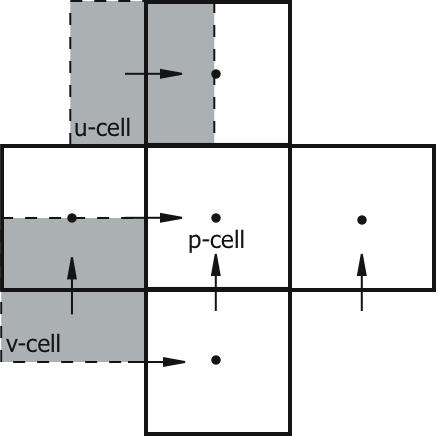
\includegraphics[width=.45\textwidth]{staggered_grid.png}
   \caption{Staggered grid arrangement in two dimensions with u and v velocity cell centers located on the face centers of the scalar cells.}
   \label{fig:staggered_grid}
   \end{center}
   \vspace{-40pt}
\end{wrapfigure}
%

%
The set of filtered equations (Equations
\ref{eqn:filtered_mass_balance}-\ref{eqn:filtered_heat_balance}) are
discretized in space and time and solved on a staggered, finite volume
mesh.  The staggering scheme consists of four offset grids. One grid
stores the scalar quantities and the remaining three grids store each
component of the velocity vector. The velocity components are situated
so that the center of their control volume is located on the face
centers of the scalar grid in their respective direction.  Figure
\ref{fig:staggered_grid} shows an example of a two-dimensional grid
and the staggering arrangement.

The staggering arrangement is advantageous for computing low-Mach LES
reacting flows.  First, since a pressure projection algorithm is used,
the velocities are exactly projected without interpolation error
because the location of the pressure gradient coincides directly with
the location of the velocity storage location. Second, Morinishi et
al. \cite{morinishi98} showed that kinetic energy is exactly conserved
when using a central differencing scheme on the convection and
diffusion terms without a subgrid model and in combination with a
staggered grid.  Having a spatial scheme that conserves kinetic energy
is advantageous because it limits artificial dissipation that arises
from the differencing scheme.  These conservation properties make the
staggered grid a prime choice for LES reacting flow simulation.

For the spatial discretization of the LES scalar equations, flux
limiting and upwind schemes for the convection operator are used.
These schemes are advantageous for ensuring that scalar values remain
bounded.  For the momentum equation, a central differencing scheme for
the convection operator is used.  All diffusion terms are computed
with a second order approximation of the gradient.

When computing the 2d surface filtered field on the faces of the
control volume, one is forced to use an interpolation from the 3d
volume filtered field.  This approximation is tolerated because
computing the 2d surface field is simply not possible with the given
grid
scheme. % This is a good example of how LES modeling issues and discrete numerics issue intertwine in applied LES modeling.

%Jennifer edited
An explicit time stepping scheme is chosen.  A general, multistep
explicit update for a variable, $\phi$, may be written as,
%
%===== Explicit Update =====
\begin{eqnarray}\label{eqn:forward_euler}
\phi^0 = \phi^n \; , \nonumber \\
  \phi^{(i)} = V \sum_{k=0}^{m-1}
\left( \alpha_{i,k}  \phi^{(k)} +
\Delta t \beta_{i,k} L( \phi^{(k)}) \right) \; , \; \; \; \; i = 1, ..., m \\
\phi^{(m)} = \phi^{n+1} \; , \nonumber
\end{eqnarray}
%
where $n$ is the time level, $m$ is the substep between $n$ and $n+1$, $\alpha$ and $\beta$ are integration coefficients, and $L$ is a linearization operator on the the convective flux and source terms.
%
Letting $m=1$ and $\alpha = \beta = 1$ the forward-Euler time
integration scheme is determined,
%%
%%===== Forward Euler =====
\begin{equation}\label{eqn:forward_euler}
\left(  \phi \right)^{n+1} = \left(
\phi \right)^{n} + \Delta t (L( \phi)^n) \; .
\end{equation}
%%
A higher order, multistep method is derived by letting $m > 1$ and
choosing appropriate constants for $\alpha$ and $\beta$. For this
study, two step and three step, strong stability preserving (SSP)
coefficients were chosen from Gottlieb et al.
\cite{Gottlieb75}.

Using the coefficients given by Gottlieb et al., the SSP-RK 2 stepping scheme is
%%
%%===== second order time stepping =====
\begin{eqnarray}\label{eqn:rk_second_order}
( \phi)^{(1)} = ( \phi)^{n} + \Delta
t (L(\phi)^n) \\ \nonumber
( \phi)^{n+1} = \frac{1}{2}(
\phi)^{n} + \frac{1}{2}( \phi)^{1} +
\frac{1}{2}\Delta t (L( \phi)^{(1)}) \;.
\end{eqnarray}
%%
SSP-RK 3 time stepping scheme is,
%%
%%===== third order time stepping =====
\begin{eqnarray}\label{eqn:rk_second_order}
(\phi)^{(1)} = (\phi)^{n} + \Delta t (L(\phi)^n) \\ \nonumber
(\phi)^{(2)} = \frac{3}{4}(\phi)^{n} + \frac{1}{4}( \phi)^{(1)} +
\frac{1}{4}\Delta t (L( \phi)^{(1)}) \\ \nonumber ( \phi)^{(n+1)} =
\frac{1}{3}(\phi)^{n} + \frac{2}{3}(
\phi)^{(2)} + \frac{1}{4}\Delta t (L(
\phi)^{(2)}) \; .
\end{eqnarray}
%%

The time step is limited by
%
\begin{equation}
\Delta t \leq c \Delta t_{F.E.}
\end{equation}
%
where $\Delta t_{F.E.}$ is the forward-Euler time step limited by
the Courant-Friedrichs-Levy condition and $c$ is a constant less
than or equal to one.  

A higher order, multistep method is derived by letting $m > 1$ and choosing appropriate constants for $\alpha$ and $\beta$. For this study, two step and three step, strong stability preserving (SSP) coefficients were chosen from Gottlieb et al. \cite{Gottlieb75}.  The coefficients for SSP-RK 2 and SSP-RK 3 are optimal in the sense that the scheme is stable when $c=1$ if the forward-Euler time step is stable for hyperbolic problems.  In practice, for the Navier-Stokes equations, the value of $c$ is taken less than one.

Choosing an explicit time stepping scheme, rather than an implict one, creates a challenge for solving the set of equations.  The density at the $n+1$ timestep, which is required to determine the cardinal variables,  requires an estimation.  Taking the estimated density for  $\overline{\rho}^{n+1}$ to be $\overline{\rho}^*$, the estimation can be as simple as $\overline{\rho}^* = \overline{\rho}^n$.  Note that the 2d and 3d filter distinction is dropped for the remainder of this discussion for the sake of simplicity.  A slightly more complicated procedure involves a forward-Euler step of the continuity equation to obtain $\overline{\rho}^*$.  This is written as,  
%
\begin{equation}\label{eqn:rho_update}
\overline{\rho}^{ *} = \overline{\rho}^{ n} - \Delta t \frac{S_k}{V} n_{kj} \left(  \overline{\rho} \widetilde{u_j} \right) \; .
\end{equation}
%
Ideally, one would like to know $\overline{\rho}^{n+1}$ rather than an
estimate.  While more details will be discussed in Section
\ref{sec:combust_react_models}, one recognizes that $\rho$ is a
function of the same variables that are being updated in time, namely,
the mixture fraction, $f$, and enthalpy, $h$.  This quandary is a
result of the explicit time stepping method will not be resolved for
variable density flows without using a fully implicit method.
Explicit methods, however, do have advantages, especially for large
scale parallel computations.  Specifically, explicit methods are
easier to load balance because the amount of work required for each
processor is readily determined a priori, which makes for an efficient
parallel computation.  Explicit methods are also easier to code into a
computer and to debug.  For these reasons, the current algorithm
discussion is limited to explicit methods only.

The explicit algorithm for solving the set of filtered equations is shown in Algorithm \ref{alg:LES_algorithm}.  
%
\begin{lstlisting}[float, caption = Explicit LES algorithm, label=alg:LES_algorithm]
for t:=t_{min} to t_{max} do 
fill in later..
for $RK_{step}$:=1 to $N$
end;
end; 
\end{lstlisting}
%
%\begin{algorithm}[t]
%\caption{Explicit LES algorithm.}\label{alg:LES_algorithm}
%
%\begin{algorithmic}[] %add [1] for #'s
%\FOR{$t = t_{min}...t_{max}$}
%\FOR{$RK_{step} = 1$...$N$} 
%\STATE 	Solve for scalars products $(\overline{\rho} \widetilde{f})^{n+1}$ and $(\overline{\rho} \widetilde{h})^{n+1}$.
%\STATE	Estimate $\overline{\rho}^* = \overline{\rho}^{n+1}$ from Equation \ref{eqn:rho_update}
%\IF{$\overline{\rho}^* < \overline{\rho}_{min}$ or $ \overline{\rho}^* > \overline{\rho}_{max}$}
%\STATE $\overline{\rho}^* = \overline{\rho}^{n}$
%\ENDIF
%\STATE Compute $\widetilde{f}^{n+1} = (\overline{\rho}\widetilde{f})^{n+1}/{\overline{\rho}^*}$ and $\widetilde{h}^{n+1} = (\overline{\rho}\widetilde{h})^{n+1}/{\overline{\rho}^*}$ 
%\STATE Compute $\overline{\rho}^{n+1} = f(\widetilde{f}^{n+1}, \widetilde{h}^{n+1})$
%\STATE Compute $\widetilde{\mathbf{u}}^*$, the unprojected velocities
%\STATE Perform RK averaging if needed
%\STATE Compute correct pressure from pressure poisson equation
%\STATE Project velocities with correct pressure to get $\widetilde{\mathbf{u}}^{n+1}$ 
%\ENDFOR
%\ENDFOR
%\end{algorithmic}
%\end{algorithm}

\section{Uintah Specification}
%
\subsection{Basic Inputs}
%
In order to run the the Arches component, the correct specification must be made for the simulation controller using the {\it SimulationComponent} tag.  In this case (similar to the other Uintah components) the Arches component is specified as
%
\begin{Verbatim}[fontsize=\footnotesize]
<SimulationComponent type="arches" />
\end{Verbatim}
%
as a child of the {\it Uintah\_specification} section.  

Most other Arches specifications are located in the {\it CFD$\rightarrow$ARCHES} section of the input file.  Unless otherwise specified, the system of units for all Arches input parameters are SGI. 

 \subsection{Time Integrator}
 % 
 \subsubsection{Explicit Time Integrator}
 Arches is commonly run in a fully explicit time-stepping mode.  That is, the update in time for any variable $\phi$ is expressed as
 %
 \begin{equation}
 \phi^{t+\Delta t} = \frac{1}{\rho^*}\left( (\rho\phi)^t +  \Delta tRHS^t) \right) \;,
 \end{equation}
 %
where  $RHS$ represents all forcing terms in the transport equation for $\phi$ at time level $t$.  For the purposes of this discussion, we have dealt with the implicit nature of the density term by simply assuming we have a density approximation, called $\rho^*$, that suits the current update (for details of the $\rho$ issue, see Section  \ref{Sec:LES_Algorithm}).  

The explicit time integrator is activated (as a child node of {\it CFD$\rightarrow$ARCHES}) by simply inserting the $<$ExplicitIntegrator$>$ node.  Within this node,  the other solvers for the various transport equations will be defined along with a few parameters.  The general structure will look something like this:
%
\begin{Verbatim}[fontsize=\footnotesize]
<ExplicitSolver>
	   <!--Solver Options-->
	   <option-1/>
	   <option-2/>
	   ....
	   <!--Transport Equations-->
	<MomentumSolver>
	...
	</MomentumSolver>
	
	<PressureSolver>
	...
	</PressureSolver>
	
	<MixtureFractionSolver>
	...
	</MixtureFractionSolver>
	
	<EnthalpySolver>
	...
	</EnthalpySolver>
</ExplicitSolver>
\end{Verbatim}  
%
The options for each transport equation will be described in Section \ref{Sec:Eqns_options}. 

Options for the $<$ExplicitSolver$>$ section include:
\begin{enumerate}
%
\item {\bf Initial time step}: $<$initial\_dt$>$ \\
{\bf Input type}: {\it Required, double} \\
{\bf Default}: {\it NA } \\ 
{\bf Description}: The explicit solver can be stepped forward in time by using a fixed time step or letting the code estimate a time step via a CFL condition (see Section \ref{Sec:LES_Algorithm}).  In either case, an initial time step must be specified. 
%
\item {\bf Variable time step}: $<$variable\_dt$>$ \\
{\bf Input type}: {\it Required, boolean} \\
{\bf Default}: {\it NA } \\ 
{\bf Description}: One may either step at a fixed time step with $\Delta t$ equal to the {\it intial\_dt} tag or let the code guess a stable time step according to a CFL condition. It is recommended that one sets the {\it variable\_dt} to {\it true}  as it helps maintain stability during the time integration.
%
\item {\bf Time integration order}: $<$timeIntegratorType$>$ \\
 {\bf Input type}: {\it Required, string} \\
 {\bf Default}: {\it FE}  \\  
 {\bf Description}: Current options include one of the following: \\ 
 \begin{itemize}
  \item FE, 1st order Forward-Euler 
  \item RK2SSP, Second Order, Strong-Stability Preserving Runge-Kutta 
  \item RK3SSP, Third Order, Strong-Stability Preserving Runge-Kutta 
 \end{itemize}
 See Section \ref{Sec:LES_Algorithm} for full details.
 % 
\item {\bf Stability option for the density guess}: $<$restartOnNegativeDensityGuess$>$ \\
 {\bf Input type}: {\it Optional, boolean} \\
 {\bf Default}: {\it false} \\
 {\bf Description}: This parameter restarts a time step, regardless of the time integrator order, if the predicted density guess (see Section \ref{Sec:LES_Algorithm}) from the continuity equation is  negative and therefore unphysical.  If this option is true, the time step is reduced by half and the time step is restarted with the new, smaller time step.  The process with repeat until a) the density guess is physical or b) the code goes unstable.  Instability usually will occur in the implicit pressure projection.  If b) occurs, it is advised to set this option to {\it false}.  By default this option is {\it false} and is not required.  Note that in cases where this parameter is {\it false} and a negative density guess occurs, the density from the previous time step is used.   
 %
\item {\bf  Message control on density guess}: $<$NoisyDensityGuess$>$ \\
{\bf Input type}: {\it Optional, boolean} \\
{\bf Default}: {\it true} \\
{\bf Description }: The negative density guess warning prints for every cell with a negative density guess.  One may want to suppress the warning and can do so with this option.  When used, a warning is printed for every patch rather than every cell.  
\item {\bf Turbulence model calculation frequency}: $<$turbModelCalcFreq$>$ \\
{\bf Input type}: {\it Optional, integer} \\
{\bf Default}: {\it 1} \\ 
{\bf Description}: This parameter allows one to control the frequency of the execution of the turbulence model.  One may want to decrease the frequency for efficiency reasons.  
\item {\bf Turbulence model calculation frequency on time integrator sub-steps}: \newline $<$turbModelCalcForAllRKSteps$>$ \\
{\bf Input type}: {\it Optional, boolean} \\
{\bf Default}: {\it true } \\ 
{\bf Description}: If {\it false}, the turbulence closure will only be computed for the first time sub-step and then applied for all subsequent time sub-steps.  By default, this parameter is {\it true}.  
\item {\bf Additional time step constraint}: $<$scalarUnderflowCheck$>$ \\
{\bf Input type}: {\it Optional, boolean} \\
{\bf Default}: {\it false}   \\ 
{\bf Description}: Guaranteeing stability for a problem with large length and time scales is difficult.  As previously mentioned, a guess at a stable time step is made using a CFL condition.  The scalar underflow check option uses additional information about the local flow information to compute an additional time step guess.  The minimum of this estimation and the CFL condition is used to step the equations forward in time.  Here, a time step is computed from the inverse of the continuity equation by considering outward mass fluxes only.  In other words, given the local velocity state, there is a limit to the amount of mass that can leave any given cell.  This limit is computed from
\[
\frac{\partial \rho}{\partial t} = -\nabla \cdot (\rho U)|_{+}
\]
when only outward facing fluxes are considered (as indicated by the $|_+$ symbol).  Thus one can rearrange this equation to give an estimate for $\Delta t$ as, 
\[ 
\Delta t \approx \partial t =  \frac{\partial \rho}{  \nabla \cdot (\rho U)|_{+}}
\] 
This option is often helpful in helping with stability if your simulation is experiencing underflow ($<1.0$) or overflow ($>1.0$) errors from the mixture fraction scalar.  
%
\item {\bf Extra pressure projection option}: $<$extraProjection$>$ \\
{\bf Input type}: {\it Optional, boolean} \\
{\bf Default}: {\it false}   \\ 
{\bf Description}: This option performs a second pressure solve and projection step.  In general, this option is not needed. By default the value is {\it false}.   
 \end{enumerate}

\subsubsection{Implicit Time Integrator}
%
Currently the implicit time integrator is not supported. Please check back in subsequent releases.

\subsection{Transport Equation Options}\label{Sec:Eqns_options}
In the current configuration of Arches, transport equations are activated by specifying the option for each equation in a equation-specific node under the {\it ExplicitSolver} node.  Currently, all equation nodes are required except for the enthalpy solver node.  

\subsubsection{Momentum Solver}
The moment solver refers to solution of $\rho \mathbf{U}$, where $\mathbf{U}$ is the vector quantity of velocity.  As mentioned above, the components are solved in a staggered, finite volume configuration. By default, the required $<$MomentumSolver$>$ node must be present in the $<$ExplicitSolver$>$ node.   

The options for the moment solver include:
\begin{enumerate}
%
\item {\bf The order of the convection scheme}: $<$convection\_scheme$>$ \\
{\bf Input type}: {\it Required, string} \\
{\bf Default}: {\it NA } \\ 
{\bf Description}: The two options that currently are implemented for the convection term in the moment equation are first-order upwind (set as {\it upwind}) and second-order central difference (set as {\it central}).  Both types of discretization can be found in any common CFD text.  It is recommended that one use the {\it central} option as it has desirable energy conservation properties (see Moronishi [add reference] ).  
%
\item {\bf Filter the divergence of $\rho \mathbf{U}$}: $<$filter\_divergence\_constraint$>$ \\
{\bf Input type}: {\it Optional, boolean} \\
{\bf Default}: {\it false } \\ 
{\bf Description}: This options turns on the filtering of the divergence constraint used in the pressure solver. When false, the divergence is unfiltered.  
%
\end{enumerate}

\subsubsection{Pressure Solver}
Arches is solved in an incompressible manner, in the sense that there is a degree of pressure-velocity decoupling which is resolved through an implicit pressure projection.  This results in the classic Poisson equation for pressure than requires solution.  By default, the required $<$PressureSolver$>$ node must be present in the $<$ExplicitSolver$>$ node.

The options for the pressure solver include:
%
\begin{enumerate}
%
\item {\bf Perform only the last projection}: $<$do\_only\_last\_projection$>$ \\
{\bf Input type}: {\it Optional, boolean} \\
{\bf Default}: {\it false } \\ 
{\bf Description}: For multi-step time schemes, only perform the projection on the last time sub-step. The result is that intermediate time steps do not conserve mass. 
%
\item {\bf Normalize the pressure with the reference pressure}: $<$normalize\_pressure$>$ \\
{\bf Input type}: {\it Optional, boolean} \\
{\bf Default}: {\it false } \\ 
{\bf Description}: When true, this option subtracts the reference pressure, set in $<$PhysicalProperties$>$, from the current value of pressure for each time step.  
%
\item {\bf Solver choice for the pressure Poisson equation}: $<$linear\_solver$>$ \\
{\bf Input type}: {\it Required, string} \\
{\bf Default}: {\it NA } \\ 
{\bf Description}: Arches uses external linear solver packages to solve the pressure Poisson equation.  Currently, there are two solver that have an interface to the pressure equation; {\it hypre} or {\it petsc}.  A solver must be specified and specifics of the solver follow in the $<$parameter$>$ section (detailed next).     
%
\item {\bf Solver parameters for the pressure Poisson equation}: $<$parameters$>$ \\
{\bf Input type}: {\it Required, NA} \\
{\bf Default}: {\it NA } \\ 
{\bf Description}: The solver parameters, as children of the {\it parameters} node, include the following:
 \begin{itemize}
 \item $<$solver$>$, Required solver parameter.  Options include: {\it cg}.  
 \item $<$max\_iter$>$, Required maximum iterations for the solver.
 \item $<$preconditioner$>$, Required preconditioner.  Options include: {\it jacobi}, {\it pfmg}. 
 \item $<$res\_tol$>$, Required tolerance of the residual ($res = b-Ax$).
\end{itemize}  
%
\end{enumerate}   
%

\subsubsection{Mixture Fraction Solver}
Arches has identified specific scalar variables that require specification, the mixture fraction being one of them.  The mixture fraction equation is a conserved scalar equation that is used as a parameter to map the thermo-chemical state of the gas.   By default, the required $<$MixtureFractionSolver$>$ node must be present in the $<$ExplicitSolver$>$ node.

\begin{enumerate}
%
\item {\bf Initial value of of the mixture fraction in the domian}: $<$initial\_value$>$ \\
{\bf Input type}: {\it Optional, double} \\
{\bf Default}: {\it 0.0 } \\ 
{\bf Description}: One may set the mixture fraction everywhere inside the domain to a constant value.  Boundary condition values are set elsewhere. 
%
\item {\bf Convection scheme}: $<$convection\_scheme$>$ \\
{\bf Input type}: {\it Required, string} \\
{\bf Default}: {\it central-upwind, flux-limited } \\ 
{\bf Description}: 
%
\end{enumerate}

\subsubsection{Enthalpy Solver}

\subsection{Initial and Boundary Conditions} 

\subsection{Turbulence Models}

\subsection{Properties, Reaction and Sub-Grid Mixing}

\subsection{Extra Scalar Solvers}
This section and all options will soon be replaced with Section \ref{Sec:AddTransEqn}. 

\subsection{Additional Transport Equations}\label{Sec:AddTransEqn}

\subsection{Direct Quadrature Method of Moments (DQMOM)}






%\subsubsection{Turbulence}


%\subsubsection{Properties}


%\subsubsection{BoundaryConditions}


%\subsubsection{Physical Constants}


%\subsubsection{Solvers}

\newpage
\section{Examples}

The following ARCHES examples illustrate the diverse set of problems that can be solved using the ARCHES component of Uintah code.  The first two examples exemplify techniques used to verify various ARCHES algorithms that were implemented in the code.  The following three [or more] examples illustrate the kinds of problems that ARCHES can solve.  The input files used here can be used as templates to build similar input files for similar problems. 
Due to the complexity of ARCHES simulations, exact solutions (with the exception of MMS) do not exist.  Hence the emphasis on model validation, or the comparison of simulation with experimental results.  Model validation provides a framework that allows the simulation scientist to be confident in his or her results in the absence of analytical solutions.  All modeling should be accompanied by some form of validation analysis.


\subsection*{\center Almgren MMS}
\addcontentsline{toc}{subsection}{Almgren MMS}
\subsubsection*{\underline{Problem Description}}

Methods of Manufactured Solutions (MMS) are verification tools that are used with computer codes such as ARCHES that seek to solve the Navier-Stokes Equations.  They are extremely useful for finding programming errors and ensuring expected behavior of the computer code.   The Almgren MMS is especially easy to implement because of the absence of source terms that must be added to the transport equations.
ARCHES uses a second-order spatial discretization scheme and a first-order scheme in the temporal direction.  Therefore, if the Almgren MMS problem is run in Arches at different mesh resolutions and the normalized error plotted on a semilog plot, the slope of the line should be 2.  To facilitate this exercise, a shell script has been written to perform this analysis \bf{[not done yet....]}  %COMPLETE ME

\subsubsection*{\underline{Simulation Specifics}}
\begin{description} 
\footnotesize
\item [Component used:] \hfill ARCHES
\item [Input file name:] \hfill \TT{almgrenMMS.ups}\\
\item [Command used to run input file:]\hfill \\

% Write .sh script to run almgrenMMS.ups 4 times at different resolutions [32,32,8], [24,24,8]. [12,12,8], and [8,8,8] and then extract L2norms to a .dat file that can easily be plotted in Excel or Matlab.
\TT{./runAlmgren.sh }

If you examine the shell script you will see the following line of code:
\TT{mpirun -np 1 sus  inputs/UintahRelease/ARCHES/almgrenMMS.ups}
This is call to run the ARCHES via sus.

\item [Simulation Domain:]\hfill    1.0 x 1.0 x 3.0 m
\item [Cell Spacing:]\hfill \\ 
0.3125 x 0.3125 x 0.275 m

\item [Example Runtimes:] \hfill \\
113.2 seconds (1 processor, 2.4 GHz Intel Core 2)

\item [Physical time simulated:] \hfill 1.0 sec.
\end{description}

%%%%%%%%%%%%%%%%%%%%%%%%%%%%%%%%%%%%
% Figure showing plot of error as a function of spatial discretization
 %%%%%%%%%%%%%%%%%%%%%%%%%%%%%%%%%%%%
 
 %--------------------------------------------------------------
 \newpage
\subsection*{\center Periodic Box Problem}
\addcontentsline{toc}{subsection}{Periodic Box Problem}
\subsubsection*{\underline{Problem Description}}
\normalfont The Periodic Box Problem indicates how well ARCHES is
modeling the kinetic energy contained in the turbulence modeled on the
grid and at a sub-grid level.  The LES algorithm transfers kinetic
energy from cell to cell in the ARCHES structured grid. Turbulence
models such as "compdynamicprocedure," "dynamicprocedure," and
"smagorinsky" are used to model kinetic energy at the sub-grid level.
Ideally, there would be a seamless transition between the resolved
turbulence and sub-grid models at the Nyquist limit.  \bf{SHOW SAMPLE
  PLOT} \normalfont Experience has shown that this is not normally the
case.  By plotting the kinetic energy as a function of the wave
number, it is possible to determine how well the kinetic energy
dissipation is being modeled by the code.  The Periodic Box problem is
initialized with a kinetic energy (turbulence) profile from Direct
Numerical Simulation (DNS).  As the simulation proceeds that energy is
dissipated.
 % COMPLETE ME

\subsubsection*{\underline{Simulation Specifics}}
\begin{description} 
\footnotesize
\item [Component used:] \hfill ARCHES
\item [Input file name:] \hfill \TT{periodic.ups}\\
 
\item [Command used to run input file:]\hfill \\
This simulation, like many ARCHES simulations, requires another file, in addition to the input file called by sus.  That file is the initial condition called upon in periodic.ups by %<set\_initial\_condition inputfile\="iso\_ini\_32.dat"/>

\TT{mpirun -np 1 sus  inputs/UintahRelease/ARCHES/periodic.ups  }  % I am using the periodic.ups file found in the tree

\item [Simulation Domain:]\hfill    0.565 x 0.565 x 0.565 m
\item [Cell Spacing:]\hfill \\ 
0.0177 x 0.0177 x 0.0177 m  %[32]^3

\item [Example Runtimes:] \hfill \\
2 minutes   (1 processor, 2.4 GHz Intel Core 2 )

\item [Physical time simulated:] \hfill 0.1 sec.  % Is this time long enough???
\end{description}

%%%%%%%%%%%%%%%%%%%%%%%%%%%%%%%%%%%%
% Figure showing plot of kinetic energy as a function of the wave number
%
% +  Discussion
%
 %%%%%%%%%%%%%%%%%%%%%%%%%%%%%%%%%%%%

 %--------------------------------------------------------------
\newpage
\subsection*{\center Helium Plume}
\addcontentsline{toc}{subsection}{Helium Plume}
\subsubsection*{\underline{Problem Description}}
Helium plumes are classical experiments that allow for the easy capture of turbulent mixing data that can be used to validate the turbulent mixing models used in LES algorithms such as Arches.  The non-reacting nature of the plume makes it easy to capture experimental data without damaging expensive equipment.  Reacting flows require special mixing tables that contain temperature, pressure and composition as a function of the transported scalars in Arches.  The coldFlowMixingModel is used to determine the mixing of \bf{isothermal?} streams. \normalfont After the mixing model is specific in the .ups file, the temperature and densities of the two mixing streams are specified.

\subsubsection*{\underline{Simulation Specifics}}
\begin{description} 
\footnotesize
\item [Component used:] \hfill ARCHES
\item [Input file name:] \hfill \TT{helium\_1m.ups}\\
 
\item [Command used to run input file:]\hfill \\
\TT{mpirun -np 8 sus  inputs/UintahRelease/ARCHES/helium\_1m.ups  }

\item [Simulation Domain:]\hfill    3.0 x 3.0 x 3.0 m
\item [Cell Spacing:]\hfill \\ 
0.06 x 0.06 x 0.0.6 m

\item [Example Runtimes:] \hfill \\
 54 minutes   (8 processors, 2.8 GHz Xeon)

\item [Physical time simulated:] \hfill 5.0 sec.
\end{description}

\subsubsection*{\underline{Results}}

%%%%%%%%%%%%%%%%%%%%%%%%%%%%%%%%%%%%
% Image from [300]^3 simulation
%
% Plot from Diem's work with the Sandia Helium Plume dataset
%%%%%%%%%%%%%%%%%%%%%%%%%%%%%%%%%%%%

 %--------------------------------------------------------------
\newpage
\subsection*{\center Methane Plume}
\addcontentsline{toc}{subsection}{Methane Plume}
\subsubsection*{\underline{Problem Description}}
This methane plume is geometrically identical to the Helium Plume problem.  The difference is the addition of chemistry.  Instead of unreacting, isothermal fluids mixing, a fuel is reacting to combustion products inside of the computational domain.  This chemistry is captured via a mixing table.  The input file is pointed to the mixing table which contains state variables and species mass fractions as a function of mixture fraction, heat loss, and mixture fraction variance.   

\subsubsection*{\underline{Simulation Specifics}}
\begin{description} 
\footnotesize
\item [Component used:] \hfill ARCHES
\item [Input file name:] \hfill \TT{helium\_1m.ups}\\
Note that the input file is pointed to the mixing table (inputs/UintahRelease/ARCHES/CH4\_equil\_clipped.mxn.gz)
 
\item [Command used to run input file:]\hfill \\
\TT{mpirun -np 8 sus  inputs/UintahRelease/ARCHES/helium\_1m.ups  }

\item [Simulation Domain:]\hfill    3.0 x 3.0 x 3.0 m
\item [Cell Spacing:]\hfill \\ 
0.06 x 0.06 x 0.0.6 m

\item [Example Runtimes:] \hfill \\
 2 hours 10 minutes   (8 processors, 2.8 GHz Xeon)

\item [Physical time simulated:] \hfill 5.0 sec.
\end{description}

\subsubsection*{\underline{Results}}
% Discussion of ...?

%%%%%%%%%%%%%%%%%%%%%%%%%%%%%%%%%%%%%
% Nifty manta image with realistic looking flame
% Specify characteristics of simulation
%%%%%%%%%%%%%%%%%%%%%%%%%%%%%%%%%%%%%

 %--------------------------------------------------------------
\newpage
\subsection*{\center Fast Cookoff}
\addcontentsline{toc}{subsection}{Fast Cookoff}
\subsubsection*{\underline{Problem Description}}
The Fast Cookoff test is a procedure used for hazard classification of energetic materials.  The object is immersed over a jet fuel pool fire and the reaction, if any, is observed.  Current protocol requires that the full size article must be subjected to this test, making such procedures prohibitively expensive and unfeasible for articles such as solid rocket motors.  An alternative procedure has been proposed, combining sub-scale experiments with computer simulation.  Through validation and uncertainty quantification procedures, the computer simulation tool (ARCHES) can be used as a surrogate for full-scale experimental testing.  This Fast Cookoff problem includes a reacting flow as well as an MPMARCHES object.  After performing the simulation, the incident heat flux to the cylinder can be extracted.  

\subsubsection*{\underline{Simulation Specifics}}
\begin{description} 
\footnotesize
\item [Component used:] \hfill MPMARCHES

\item [Input file name:] \hfill \TT{fastcookoff.ups}\\

\item [Command used to run input file:]\hfill \\
Note that the input file is pointed to the mixing table (inputs/UintahRelease/ARCHES/sandia\_jp8\_flmlt\_cg.mxn)

\TT{mpirun -np 64 sus  inputs/UintahRelease/ARCHES/fastcookoff.ups  }
To extract the incident heat flux to the cylinder, use the faceextract and timeextract utilities.  <How to do this>

\item [Simulation Domain:]\hfill    24.0 x 24.0 x 24.0 m
\item [Cell Spacing:]\hfill \\ 
0.24 x 0.24 x 0.24 m

\item [Example Runtimes:] \hfill \\
7 hours 27 minutes   (64 processors, 2.8 GHz Xeon)  % UDA at /scratch/uintah/hinckley/ARCHES_examples

\item [Physical time simulated:] \hfill 10.0 sec.
\end{description}

\subsubsection*{\underline{Results}}


%\section{References}
\bibliographystyle{plain}
\bibliography{arches}
